\pagebreak
\chapter{Philosophy of Science} 
\setcounter{section}{0}

\section{Karl Popper}

\subsection{Einführung}



\subsection{Logik der Forschung - 1934}
\subsubsection{Falsifizieren}
\paragraph{Verifizieren vs Falsifizieren}
Das mit Karl Popper hervorgebrachte Grundprinzip ist: \textit{Theorien sind nicht zu beweisen, sondern zu wiederlegen.}\\

\textbf{Zum Beispiel:} Die Theorie sagt, alle Schwäne sind weiß. Dann sollte das Ziel sein, nicht weiße Schwäne zu finden. Das Ziel, weiße Schwäne zu finden, ist kein ausreichendes.\\

\textbf{Zum Beispiel:} \textit{Macht Kaffee die Haut schön.} Es kann gegoogelt werden, ob Kaffee die Haut schön macht (Verifizieren). Die Fasizifierung sieht aus, dass nach Gegenbeweisen gesucht wird: Macht Kaffee die Haut nicht schön.

\paragraph{Was macht eine Hypothese aus}
Zwei Kriterien sind für eine Hypothese entscheidend
\begin{itemize}
	\item Eine Hypothese ist wissenschaftlich, wenn sie die das Potenzial besitzt durch Beweise oder Beobachtung widerlegt zu werden.
	\item Eine Hypothese muss \textit{riskant} sein.
\end{itemize}

Der letzte Punkt Ziel darauf ab, dass eine Hypothese vermeiden soll, mit allen Beobachtungen übereinzustimmen. Dazu muss bei der Wahl einer Hypothese Risiken eingegangen werden. Denn erst so, besteht die Chance neue Erkenntnisse zu gewinnen oder auch widerlegt zu werden.

\paragraph{Pseudo-Science vs. Science}
Die Unterscheidung zwischen Pseudo und normalen Wissenschaften wird in dem Kontext nicht als für und wider angesehen. Es soll lediglich eine Unterscheidung geben, wie Wissen gewonnen werden kann und wie dies nicht funktioniert.\\

Ein Beispiel für Pseudo-Science ist $"$Freuds Theory$"$. Egal welche Beobachtung getroffen wird, die Theory kann es klären. Eine Theory muss $"$Risiken$"$ eingehen. Dies bedeutet nicht, dass es Beobachtungen gibt, welche nicht zu treffen, sondern dass erkenntlich ist, welche \textit{möglichen Beobachtungsscenarien} nicht mit der Theory kompatible sind.

\subsubsection{Wissenschaftlicher Fortschritt/ Scientific Change}

\paragraph{Eigenschaften eines Wissenschaftlers}

 A Great Scientist
“A hardheaded Cowboy with a Violin”
- A creative and artistic strik
- Tough minded, no-nonsense streak - Testing an critical thinking

Those attributes can be share among a group or included in one person
- Social Structure
    - On comes up with conjectures 
    - and the other with refutation

But a good scientist tried to combine both attitudes.

In the later chapter of Theroy & Reality, the focus is, how a good setup of dividing the Labor can encure to advance the knowledge in a fast past and not get stuck.

\paragraph{Theorie Aufbau}

Das Ziel einer Theory ist, (Aim of a theory: )
- die Tiefe zu verstärken und (breadth of a theory)
- die Genauigkeit (increase the precision of its prediction) 
der Aussagen.


\paragraph{Conjecture und Falsifizieren (Zwei Schritte)} 
\begin{itemize}
	\item Conjecture (Vermutung) eine riskante und mutige Hypothese
	\item Es werden Anstrengungen unternommen, die Hypothese zu widerlegen.
\end{itemize}

Dies Art der Untersuchung ist der Zustand, welche angestrebt werden soll. Es ist nicht immer möglich, die Hypothesen zu falsifizieren. Dennoch ist der zweite Punkt, der Falsifikation, nicht ausschließlich auf die Arbeit eines Experiments gebunden. Der Grund-Tenor ist, dass man selbst, oder diese Aufgabe wird ausgelagert, 
\begin{itemize}
	\item neben einer Verifizierung immer nach Gegenbeweisen sucht,
	\item sich einer außenstehenden Testung der Hypothese unterzieht oder
	\item die Möglichkeit sucht, unter anderen Gesichtspunkten, die Hypothese widerlegen möchte.
\end{itemize}

Der letzte Punkt ist wohl der wichtigste. Die Motivation soll immer bestehen, die eigenen Theorie widerlegen zu wollen.\\

Erkenntnisse aus den Beobachtungen führen wieder zu Anpassungen im Model. Die Änderungen soll jedoch nicht wie ein Pflaster verstanden werden oder als eine Art Umfassung der Beobachtung verstanden werden (Ref: Pseudo-Science).\\ 

Das Ziel einer Theorie bleibt gleich, die Theory soll aus sich heraus eine mutige Hypothese formulieren, nicht nur zu der Observation passen.


\paragraph{Untersuchung von wissenschaftlichen Vorgehen}
Wie schon erwähnt, ist die Falsifikation nicht immer möglich, daher ist im wissenschaftlichen Kontext zu beobachten, dass nicht alle Experiment dies versuchen.
\begin{figure}[H]
	\centering
	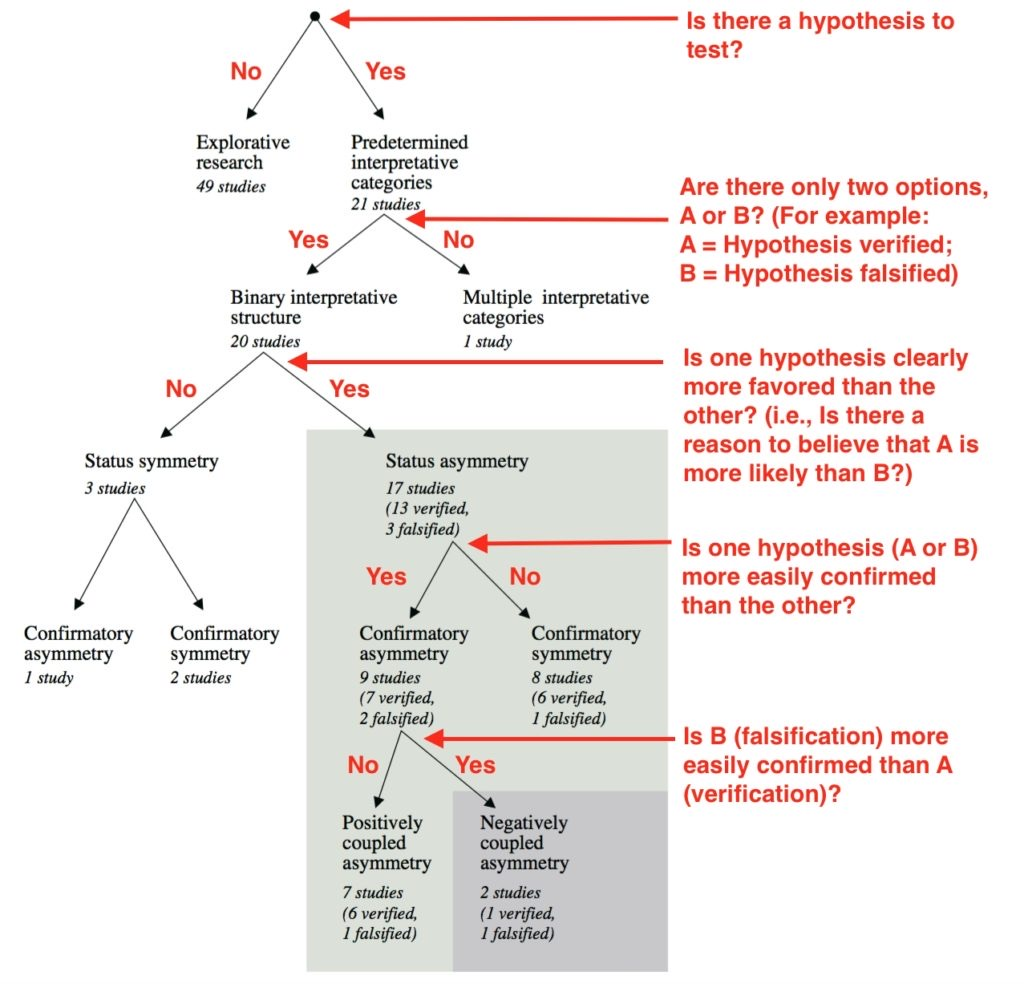
\includegraphics[scale = 0.2]{attachment/chapter_13/Scc078}
	\caption{Vorgehen von wissenschaftlicher Theorie F/V} 
\end{figure}







\subsubsection{Andere Möglichkeiten die Welt zu untersuchen}
\paragraph{Simple Empirisism}
Bei Empirisim geht es darum, dass die Beobachtung die Wahrheit ist. Postives Bsp.: Collora in London. Es wurde beobachtet, dass ein Brunnen. Ein Gegenbeispiel ist, dass ein Kollege von Pasteur ein Glas mit Batterien getrunken hat und nicht krank wurde. Vom Prinzip existiert hier auch eine Theorie. Diese war nur nicht genau genug überprüft worden. Es besteht das Problem des Beispielsatzes mit 1.

\paragraph{Explorative Suche}
Eine Explorative Suche benötigt keine Idee, sondern ist für den Theorie Bau notwendig. 

\subsection{Die Offene Gesellschaft und ihre Feinde - 1945}
Um die Frage nach eine funktionierenden Gesellschaft zu beantworten, hat Karl Popper für sich die Frage versucht zu beantworten: Was kann man wissen. Dies wurde im dem Werk: Logik der Forschung adressiert.

\subsubsection{Falsifikation Politischen Strukturen}
Eine offenen Gesellschaft muss nach Popper sicherstellen, dass die Falsifikation auf den politischen Strukturen in einer Gesellschaft gewährleistet wird.\\

Warum: Politische Strukturen sind Theorien über Soziales Handeln in einer Gesellschaft. Nur im Ansatz über (1) Conjectur (Theorie Vorschlag über Soziales Handeln) und (2) Falzifikation kann Wissen über das Soziale Handeln gewonnen werden - was funktioniert und was nicht.



\subsubsection{Macht auf Zeit}
Um den Prozess der Falsifikation politischer Strukturen (Regierungen, Institutionen) zu gewähren, ist angenommmen, dass Macht nur auf Zeit gehalten werden muss, sonst besteht das Risiko, dass selbst trotz einer Falsifikaiton einer Regierung, diese nicht nach der Falsifikation handelt, wenn es bedeutet, dass ihre Theorie über das soziale Handeln, nicht richtig ist.

Um einen Regierungen, Machthaber/ Entscheidungsträger/ Experimenter, neu besetzen zu können, muss gelten:
\begin{itemize}
	\item Machthaber müssen ohne Gewahlt abwählbar sein
	\item Regierungen, als Hüllen für Theorie, müssen neu wählbar sein.
	\item Dezentrale Macht Verteilung
\end{itemize}

Hier ist der Unterschied zu Platon. Dieser übergibt Macht auf Unbestimmt der Philosophen Rege. Für Popper ist eine Annahme, dass Macht nur begrenzt gegeben werden kann.

\subsubsection{Jeder einzelne}
\paragraph{Bewusstsein über Mehraufwand}
Der Aufbau der Offenen Gesellschaft erfordert, dass dies einen größer permanente Anstrenung von jedem Mitglied der Gesellschaft verlangt.

\begin{itemize}
	\item Eine offenen Gesellschaft ist eine instabilere Gesellschaft, im Vergleich zu einer geschlossenen Gesellschaft. Die permanente Ummodellierung und Testen erfordert Kraft und sorgt für Unsicherheit. In einer geschlossenen Gesellschaft sich die möglichen Alternativen verborgen, werden nicht debattiert oder stehen nicht zur Auswahl.
	\item Die Person steht an erster Stelle: Dies bedeutet auch, dass jeder einzelne Kritik empfangen und geben, Neue Ansätze aushalten und sich einbringen muss.
\end{itemize}

\paragraph{Tugenden}
\begin{description}
	\item[Verzeihen] Wenn kontinuierlich Kritik geübt wird, wird es so sein, dass einige $"$Hypothesen$"$ falsch sein werden. Das eine Person falsch liegt, sollte ihr verziehen wer	
	\item[Toleranz] $"$Other people are hell.$"$ Diese Zitat weißt darauf hin, dass Tolerenz, für $"$Leider ertragen/aushalten$"$, durch die Unstimmigkeit gegenüber andere Personen besteht. Bei der Toleranz kommt es jedoch darauf an, dass die Person mit der man in Unstimmigkeit noch als andere Person mit allen ihren Rechten und Pflichten in der Gesellschaft respektiert wird.
	\item[Tolerenz Grenzen] Eine Person, welche Dir nicht tolerant ist, der muss ebenso keine Toleranz entgegen gebracht werden. Somit schließt Toleranz zu sein, nicht eine Kriegshandlung aus.
	\item[Mut] Um neue Ideeen auszuprobieren, muss Mut bestehten, diese auf zuzubringen, den es besteht die Wahrscheinlichkeit, dass man falsch liegt.
\end{description}


\subsubsection{Die Feinde}

\paragraph{Geschlossenen Gesellschaft (Totalitäritäüt)}

In einer geschlossenen Gesellschaft sich andere möglichen Alternativen des Zusammenlebens verborgen, werden nicht debattiert oder stehen nicht zur Auswahl.

Mit der Erkenntnis, dass Wissen nur falzifiziert nicht verifiziert werden kann, würde sich eine geschlossenen Gesellschaft dem widerziehen.\\

Eine mögliche Verbesserung oder Anpassung ist so nicht vorgesehen.\\ 

Der Vorteil ist, dass die Entscheidungsdauer geringer ist, weil ein abgleich mit anderen Alternativen nicht benötigt ist - Man weiß ja, dass es richtig ist.

\paragraph{Utopien}
Eine Utopie ist eine $"$Pseudo-Wissenschaftliche Theorie$"$ über soziales Verhalten. Es wird mit einem simplen Ansatz viele Probleme versucht zu lösen.

Entweder kann nie überprüft werden, ob eine Utopie Wirkung zeigt oder sie umfasst alle Beobachtungen und beschreibt somit nichts eigenes.\\

Risiko: Kurzfristiges Leide wird für den $"$möglichen$"$ zukünftigen postiven Zustand in Kauf genommen.

\paragraph{Platon, Hegel und Karl-Marx}
Alle drei starten mit großen Ideen (Uptopien).
\begin{itemize}
	\item Hegel: Das Weltgesehen steigt immer positiv voran. Es exisitert ein positiver Geschichtsverlauf. 
	\item Platon: Staatstheorie; Starke Machthaber; Experten/ Philiosphen machen sich am meisten Gedanken, weshalb sie Denker Aufgaben in einer Gesellschaft übernehmen -> Kein Machtwechsel möglich. Das Problem ist Macht auf unbegrenzte Zeit.
\end{itemize}